\chapter{Learning patterns of inter-subject functional variability from data}\label{chap:func_var}
\markright{{~{\rm \ref{chap:func_var}}. Learning inter-subject functional variability from data}\hfill}{}

\minitoc

% \section{Brains are different in function}
% \section{Introduction to brain decomposition and matrix factorization / dictionary-learning}
% \label{sec:intro}
\newthought{In neuro-imaging}, inter-subject variability is often handled as a statistical residual and discarded. Yet there is evidence that it displays structure and contains important information. Univariate models are ineffective both computationally and statistically due to the large number of voxels compared to the number of subjects. Likewise,
statistical analysis of weak effects on medical images often relies on
defining regions of interests (ROIs). For instance, pharmacology
with Positron Emission Tomography (PET) often studies metabolic
processes in specific organ sub-parts that are defined from anatomy.
Population-level tests of tissue properties, such as diffusion, or
simply their density, are performed on ROIs adapted to the spatial
impact of the pathology of interest. In functional brain imaging,
e.g function magnetic resonance imaging (fMRI), ROIs must be
adapted to the cognitive process under study, and are often defined by
the very activation elicited by a closely related process  \citep{saxe2006}.
ROIs can boost statistical power by reducing multiple comparisons that
plague image-based statistical testing. If they are defined to match
spatially the differences to detect, they can also improve
the signal-to-noise ratio by averaging related signals. 
%
However, the crux of
the problem is how to define these ROIs in a principled way. 
%
Indeed, standard approaches to region definition imply a
segmentation step. 
Segmenting structures on first-level statistical maps, as in fMRI,
typically yields meaningful units, but is limited by the noise
inherent to these maps.
Relying on a different imaging modality
hits cross-modality correspondence problems.



% \chapter{Online structured unsupervised dictionary-learning}
%% \begin{abstract}
%% We propose a multivariate online dictionary-learning
%%   method for obtaining decompositions of brain
%% images with structured and sparse components (aka atoms). Sparsity is
%% to be understood in the usual sense: the dictionary atoms are
%% constrained to contain mostly zeros. This is imposed via an $\ell_1$-norm
%% constraint. By "structured", we mean that the atoms are piece-wise
%% smooth and compact, thus making up blobs, as opposed to scattered
%% patterns of activation. We propose to use a Sobolev (Laplacian)
%% penalty to impose this type of structure.
%% %
%% Combining the two penalties, we obtain decompositions that properly
%% delineate brain structures from functional images.
%% %
%% This non-trivially extends the
%% online dictionary-learning  work of Mairal et
%% al. (2010), at the price of only a factor of 2 or 3 on the overall
%% running time. Just like the Mairal et al. (2010) reference method, the
%% online nature of our proposed algorithm allows it to scale to
%% arbitrarily sized datasets. Experiments on brain data show that our proposed method extracts structured and denoised dictionaries that are more intepretable and better capture inter-subject variability in small medium, and large-scale regimes alike, compared to state-of-the-art models.
%% %% We focus on difficult parameter selection issues by introducing relevant criteria (reproducibility, explained variance, use in prediction tasks) and describe the optimality regime.
  
%% %% \textit{\textbf{Keywords:}} Inter-subject variability; MRI; multivariate methods; online dictionary-learning; large-scale learning; sparsity; spatial regularization

%% \end{abstract}
%\tableofcontents

\section{Introduction and sketch of our contributions}
\label{sec:intro}
In this manuscript, we propose to use the \textit{variability} of the statistical
maps across the population to define regions.
%
This idea is reminiscent of
clustering approaches, that have been employed to define spatial units
for quantitative analysis of information as diverse as brain fiber
tracking, brain activity, brain structure, or even imaging-genetics. See   \citep{Varol2014,hibar2013genetic} and references therein.
%
The key idea is to group together features --voxels of an image,
vertices on a mesh, fiber tracts-- based on the quantity of interest, to
create regions --or fiber bundles-- for statistical analysis. However,
unlike clustering that models each observation as an instance of a
cluster, we use a model closer to the signal, where each observation is a
linear mixture of several signals. The model is closer to mode finding,
as in a principal component analysis (PCA), or an independent component
analysis (ICA), often used in brain imaging to extract functional units
  \citep{beckmann2004}. Yet, an important constraint is that the modes
 should be sparse and spatially-localized. For this purpose, the problem can be reformulated as a linear decomposition problem like ICA/PCA, with
 appropriate spatial and sparse penalties   \citep{varoquaux2011,abraham2013}. 

We propose a multivariate online dictionary-learning method for obtaining
decompositions with structured and sparse components (aka atoms).
Sparsity is to be understood in the usual sense: the atoms contain mostly
zeros. This is imposed via an $\ell_1$ penalty on the atoms. 
%
By "structured", we mean that the atoms are piece-wise smooth and
compact, thus making up blobs, as opposed to scattered patterns of
activation. We impose this type of structure via a Laplacian penalty on the
dictionary atoms. Combining the two penalties, we therefore
obtain decompositions that are closer to known functional organization of the brain. This non-trivially extends the online dictionary-learning /
dictionary-learning work   \citep{mairal2010}, with only a factor of 2
or 3 on the running time.
%
By means of experiments on a large public dataset, we show the
improvements brought by the spatial regularization with respect to
traditional $\ell_1$-regularized dictionary learning.
%
We also provide a concise study of the impact of
hyper-parameter selection on this problem and describe the optimality
regime, based on relevant criteria (reproducibility, captured
variability, explanatory power in prediction problems).

Applied to
functional brain imaging, it separates successfully activation maps into
localized units of brain activity.
Our contribution is to frame spatial penalties as a particular case of
more general Laplacian regularization and introduce an efficient online
algorithm for dictionary-learning in these settings. Applied to
functional brain imaging, it separates successfully activation maps into
localized units of brain activity.
Here we do things that are closer to probabilistic segmentations

%% \paragraph*{Notation and terminology.} Let $\X$
%% and $\Y$ be matrices (matrices will be written in
%% bold-face) of the same size. %, and $\mathbb E$ be a finite-dimensional
%% % Euclidean space.%%  and $C$ be a closed convex subset
%% %% thereof. %% $[\![M,N]\!]$ will denote the
%% %%   %% integers from $M$ through $N$, i.e $[\![M,N]\!] := \mathbb Z \cap
%% %%   %% [M, N]  = \{M,M+1,\ldots,N\}$.
%% %%   $P_C$ denotes the Euclidean
%% %%   projection (i.e the closest-point map, w.r.t $\ell_2$-norm) operator
%% %%   onto $C$
%%   . The $k$th row of $\X$ (resp. $j$th column of $\X$ or $j$th row of its transpose $\X^T$) will be denoted $\B{x}_k$ (resp. $\X^j$).
%% $\mathrm{vec}(\X)$ will denote the concatenation of $\X$ into a single vector.
%% The Frobenius (aka Hilbert-Schmidt)
%% inner-product of $\X$ and $\Y$ is
%% defined by
%% $\langle \X, \Y\rangle_{\text{Fro}} :=
%%   \sum_{k, j}\B{x}_k^j\Y_k^j = \langle \mathrm{vec}(\X),
%%   \mathrm{vec}(\Y)\rangle.$
%% The Frobenius norm of $\X$,  is defined by
%% $$\|\X\|_{\text{Fro}} :=\sqrt{\langle \X, \X\rangle_{\text{Fro}}} =
%% \|\mathrm{vec}(\X)\|_2.$$

%% %% \item[--] \textbf{Mixed-norm.} $\|\X\|_{p,q} :=
%% %%   \sqrt[q]{\sum_{k}\|\B{x}_k\|_p^q}$. The case $p = 2$, $q = 1$
%% %%   corresponds to the usual ``group-norm'' used in the Group-Lasso
%% %%   and related models.
%% %% \item[--] \textbf{Group soft-thresholding operator.}
%% %%   $$\mathrm{gsoft}_\lambda: \mathbb{R}^{p \times d} \rightarrow
%% %%   \mathbb{R}^{d \times p}, (g_k)_{k \in [\![1,p]\!]} \mapsto \left(\left(1 -
%% %%   \lambda/\|g_k\|_2\right)_+g_k\right)_{k \in [\![1,p]\!]},$$
%% %%   where $(a)_+ := \max(a, 0)$, for $-\infty \le a \le \infty$.
%% %% \item[--] \textbf{Balls for the $\ell_p$ (mixed-) norm.} $\mathbb
%% %%   B_p(\lambda) := \{x \in \mathbb E | \|x\|_p \le \lambda\}$. For
%% %%   shorthand, The Euclidean projection onto the unit-ball $B_p(1)$ will
%% %%   be denoted $P_p$.
%% Finally, $\nabla_x$ will denote the discrete spatial gradient operator
%% along the $x$-axis, $\nabla_y$ along the $y$-axis, etc. $\Delta :=
%%   -\nabla^T\nabla$ is the $p$-by-$p$ matrix representing the discrete
%%   Laplacian.

\section{Smooth Sparse Online Dictionary-Learning (Smooth-SODL)}
\label{sec:contrib}
\begin{figure}
    \centering
    \def\svgwidth{\columnwidth}
    \input{figures/dlsvg.pdf_tex}
    \caption{...}
  \end{figure}
  
% \begin{figure}[!htp]
% \includesvg[width=1.\linewidth]{figures/dlsvg.svg}
% \end{figure}
Consider a stack $\X
\in \mathbb R^{n \times p}$ of $n$ subject-level brain images
$\B{x}_1,\B{x}_2,\ldots,\B{x}_n$ each of shape $n_1 \times n_2 \times n_3$, seen as
$p$-dimensional row vectors --with $p = n_1\times n_2 \times n_3$, the number of voxels. These could be images of fMRI activity
patterns like statistical parametric maps of brain activation, raw
pre-registered (into a common coordinate space) fMRI time-series, PET
images, etc. We would like to decompose these images as a product of
$k \le \min(n, p)$ component maps (aka latent factors or dictionary atoms)
 $\B{d}^1,
\ldots, \B{d}^k \in \mathbb{R}^{p \times 1}$ and modulation coefficients
$\B{c}_1, \ldots, \B{c}_n \in \mathbb R^{k \times 1}$ called \textit{codes} (one $k$-dimensional code per sample point), i.e
\begin{eqnarray}
\B{x}_i \approx \B{D} \B{c}_i, \text{ for } i=1,2,\ldots,n
\end{eqnarray}
where $\B{D} := [\B{d}^1|\ldots|\B{d}^k] \in \mathbb{R}^{p \times k}$, an unknown dictionary to be estimated.
Typically, $p \sim 10^{5}$ --
$10^{6}$ (in full-brain high-resolution fMRI) and $n \sim 10^{2}$ --
$10^{5}$ (for example, in considering all the 500 subjects and all
the about 15 --20 functional tasks of the Human Connectome Project dataset   \citep{VanEssen20122222}). Our work handles the extreme
case where both $n$ and $p$ are large (massive-data setting). 
%
It is reasonable then to only consider under-complete dictionaries: $k
\le \min(n, p)$. Typically, we use $k \sim 50$ or $100$ components.
%
It should be noted that online optimization is not only crucial in the
case where $n / p$ is big; it is relevant whenever $n$ is large,
leading to prohibitive memory issues irrespective of how big or small
$p$ is.

As explained in section \ref{sec:intro}, we want the component maps (aka dictionary atoms) $\B{d}^j$ to be sparse and spatially smooth. A principled way to achieve such a goal is to impose a boundedness constraint on $\ell_1$-like norms of these maps to achieve sparsity and
simultaneously impose smoothness by penalizing their Laplacian.
Thus, we propose the following penalized dictionary-learning model
\begin{eqnarray}
\begin{split}
  &\min_{\B{D} \in \mathbb R^{p \times k}}\left(\lim_{n \rightarrow \infty}\frac{1}{n}\sum_{i=1}^n\min_{\B{c}_i \in \mathbb R^{k}}\frac{1}{2} \|\B{x}_i-\B{D}\B{c}_i\|_2^2 +  \frac{1}{2}\alpha\|\B{c}_i\|_2^2\right) + \gamma\sum_{j=1}^k{\text{Lap}}(\B{d}^j).\\
  &\text{subject to }\B{d}^1,\ldots,\B{d}^k \in \mathcal C
\end{split}
% XXX: I am discovery the l1 penalty on U. Do we really need this ?
\label{eq:ss}
\end{eqnarray}
The ingredients in the model can be broken down as follows:
\begin{itemize}
\item Each of the terms $\max_{\B{c}_i \in \mathbb R^k}\dfrac{1}{2}\|\B{x}_i-\B{D}\B{c}_i\|_2^2$ measures how well the current dictionary $\B{D}$ explains data $\B{x}_i$ from subject $i$.
  %% \dfrac{1}{2n}\|\X -\B{C}\B{d}^T\|_{\text{Fro}}^2
  %% $ is the mean reconstruction error on $n$ subjects and measures how well the codes $\B{c}_1,\B{c}_2,\ldots,\B{c}_n$ approximate the data $\X$ using the current dictionary $\B{D}$, the vector $\B{x}_i-\B{D}\B{c}_i$ being the reconstruction error for subject $i$. Both the $\B{C}$ and $\B{D}$ matrices are parameters to be estimated.
The Ridge penalty term $\phi(\B{c}_i) \equiv \frac{1}{2}\alpha\|\B{c}_i\|_2^2$
amounts to placing an isotropic Gaussian prior on the codes, namely $p(\B{c}_i) \propto \exp(-\frac{1}{2}\alpha\|\B{c}_i\|_2^2)$. In the context of a specific
neuro-imaging problem, if there are good grounds to assume that each
sample / subject should be sparsely encoded across only a few atoms of
the dictionary, then we can use the $\ell_1$ penalty $\phi(\B{c}_i) :=
\alpha\|\B{c}_i\|_1$ as in   \citep{mairal2010}, corresponding to a Laplace prior on the codes, namely $p(\B{c}_i) \propto \exp(-\alpha\|\B{c}_i\|_1)$. We note that in contrast to
the $\ell_1$ penalty, the Ridge leads to stable codes. The parameter $\alpha > 0$ controls the amount of penalization on the codes. %, which can be updated in closed-form via SVD. %% (w.r.t small pertubations in the input data $\X$) due to strong-convexity of the resulting coding problem \eqref{eq:coding}.

  %% It is essential to constrain the magnitude of the codes $\B{c}_i$ to
  %% prevent them from becoming arbitrarily large, which would lead to a
  %% pathological all-zero values in the dictionary atoms, and vice versa.

  %% The proposed Laplacian penalty terms
  %% ${\text{Lap}}(\B{d}^j)$ defined in \eqref{eq:sob} imposes spatial smoothness
  %% on the dictionary atoms $\B{d}^j$, see e.g. Fig. \ref{fig:roi}.
%% \textbf{XXX I don't see what you mean here}.
\item The constraint set $\mathcal C$ is a sparsity-inducing compact
simple\footnote{Mainly in the sense that the Euclidean projection onto
$\mathcal C$ should be easy to compute.} convex subset of $\mathbb R^p$
like an $\ell_1$-ball $\mathbb B_{p,\ell_1}(\tau)$ or a simplex $\mathcal S_p(\tau)$, defined respectively as $$\mathbb B_{p,\ell_1}(\tau) := \left\{\B{d} \in \mathbb R^p\text{ s.t }|\B{d}_1| + |\B{d}_2| + \ldots + |\B{d}_p| \le \tau\right\},$$
and
$\mathcal S_p(\tau) := \mathbb B_{p,\ell_1}(\tau) \cap \mathbb R_+^p.$
Other choices (e.g ElasticNet ball) are of course possible. The radius parameter $\tau > 0$ controls the
amount of sparsity: smaller values lead to sparser atoms.
%% \item More general sparsity-inducing  constraint sets like elastic-net balls and probability simplexes can be be considered: we only require the existence of an efficient oracle for projection onto the constraint set $\mathcal C$.  
The Laplacian regularization $\text{Lap}$ (see table of notations) is meant to impose blobs.
$\gamma \ge 0$ controls how much regularization we impose on the atoms, compared to the
reconstruction error.

\end{itemize}
The above formulation, which we dub \textit{Smooth Sparse Online Dictionary-Learning} (Smooth-SODL) is inspired by, and generalizes the standard
dictionary-learning framework of   \citep{mairal2010} --henceforth referred to as \textit{Sparse Online Dictionary-Learning} (SODL); setting $\gamma = 0$, we recover SODL   \citep{mairal2010}.

% \begin{remark}
% Of course, we can accommodate a brain mask by using the masking / un-masking tricks outlined in   \citep{michel2011tv}.  
% Also, our framework extends effortlessly to arbitrary space
% dimensions, by simply considering a $D$-dimensional discrete
% finite-difference difference spatial gradient operator $\nabla =
% [\nabla_x, \nabla_y, \nabla_z,\ldots]$, in place of the 3-dimensional ($D=3$) case considered in this manuscript. Thus our methods
% can be readily applied to multiple-valued imaging modalities, such as Diffusion Tensor Imaging (DTI) data.
% \end{remark}

\subsection{Interpretation as an ``encoder-less'' generative model of brain data}
One notes that the proposed model \ref{eq:ss} can be seen as an auto-encoding model of brain data with linear generator

\begin{equation}
  G_{\B{D}} = \langle \B{D}, .\rangle: \mathbb R^k \times \mathbb R^p,\; \B{c} \mapsto \B{Dc},
\end{equation}
parametrized by the learned dictionary $\B{D} \in \mathcal C$, and an \textit{implicit} encoder
\begin{equation}
  E_{\B{D}}: \mathbb R^p \rightarrow \mathbb R^k,\; \x \mapsto \argmin_{\B{c} \in \mathbb R^k} -\text{loglik}(p(\B{c}|\x,\B{D})p(\B{c})) = \argmin_{\B{c} \in \mathbb R^k}\ell(G_\B{D}(\B{c}),\x) + \alpha\phi(\B{c}).
  \end{equation}


\section{Algorithms}
% \paragraph*{Optimizing the proposed model: a simple algorithm.}
The objective function in problem
\eqref{eq:ss} is separately convex and block-separable
w.r.t each of $\B{C}$ and $\B{D}$ but is not jointly convex in $(\B{C},\B{D})$. Also,
it is continuously differentiable on the constraint set, which is
compact and convex. Thus by classical results (e.g Bertsekas   \citep{bertsekas1999nonlinear}), the problem can be solved via
Block-Coordinate Descent
(BCD)   \citep{mairal2010}.
 Reasoning along the lines of   \citep{jenatton2010structured}, we derive
 that the BCD iterates are as given in Alg. \ref{Tab:algo}.
A crucial advantage of using a BCD scheme is that it is parameter
free: there is not step size to tune.
%e
The resulting algorithm Alg. \ref{Tab:algo}, is adapted from   \citep{mairal2010}.
It relies on Alg. \ref{Tab:algo_sobdict} for performing the structured dictionary updates, the details of which are discussed below.

\begin{algorithm}
\caption{Online algorithm for the dictionary-learning problem
  \eqref{eq:ss}}
\label{Tab:algo}
\begin{algorithmic}[1]
\Require %% Random data $x \in \mathbb R^m$ with unknown distribution
%% $p(x)$, but with an effective way of empirically sampling from this
%% distribution; 
Regularization parameters $\alpha, \gamma > 0$;
initial dictionary $\B{D} \in \mathbb R^{p \times k}$,
number of passes / iterations $T$ on the data.
\State $\A_0 \leftarrow 0 \in \mathbb R^{k \times k}$, $\B{B}_0
\leftarrow 0 \in \mathbb R^{p \times k}$ \text (historical ``sufficient statistics'')
\For{$t = 1$ to $T$}
\State Empirically draw a sample point $\B{x}_t$ at random.
\State Code update: Ridge-regression (via SVD of current dictionary $\B{D}$)
\begin{equation}
\B{c}_t \leftarrow \argmin_{\B{c} \in \mathbb R^k}\frac{1}{2}\|\B{x}_t -
\B{D} \B{c}\|_2^2 + \frac{1}{2}\alpha\|\B{c}\|_2^2.
\label{eq:coding}
\end{equation}
\State Rank-1 updates:
$\A_t \leftarrow \A_{t-1} + \B{c}_t\B{c}_t^T,\; \B{B}_t \leftarrow \B{B}_{t-1} + \B{x}_t\B{c}_t^T$
\State BCD dictionary update: Compute update for dictionary $\B{D}$ using
Alg. \ref{Tab:algo_sobdict}.
\EndFor
\end{algorithmic}
\end{algorithm}

\paragraph*{Update of the codes: Ridge-coding.}
The Ridge sub-problem for updating the codes%, namely
\begin{equation}
  \B{c}_t = (\B{D}^T\B{D} + \alpha \I)^{-1}\B{D}^T\B{x}_t
  \label{eq:code}
\end{equation}
is computed via an SVD of the current dictionary $\B{D}$.
For $\alpha \approx 0$, $\B{c}_t$
reduces to the orthogonal projection of $\B{x}_t$ onto the image of the current
dictionary $\B{D}$.
% Once this SVD is computed, the codes corresponding to a batch of inputs $\B{x}_t$ can be computed in closed-form.
As in   \citep{mairal2010}, we speed up the overall algorithm by sampling mini-batches of $\eta$ samples $\B{x}_t,\ldots,\B{x}_\eta$ and compute the corresponding codes $\B{c}_1$, $\B{c}_2$, ..., $\B{c}_\eta$ at once. We typically use we use mini-batches of size $\eta \sim 20$ images.

\paragraph*{BCD dictionary update for the dictionary atoms.}
%% \paragraph{Updating the codes.}
%% For a fixed dictionary $\B{D}$, and an incoming sample point $\B{x}_t$ at time
%% $t$, the optimization of the energy $E(\B{C}, \B{D})$ in
%% \eqref{eq:ss}, for the code can be written as
%% \begin{eqnarray}
%% \B{c}_t = \argmin_{\B{c} \in \mathbb R^k}\frac{1}{2}\|\B{D} \B{c} -
%% \B{x}_t\|_2^2 + \alpha\phi(\B{c}).
%% \end{eqnarray}
%% With the choice $\phi = \|.\|_1$, this is a sparse-coding problem   \citep{mairal2009,mairal2010} and
%% corresponds to a Lasso regression and can be effectively solved with a
%% LARS-Lasso solver. With the choice $\phi = \frac{1}{2}\|.\|_2^2$, this
%% problem corresponds to Ridge regression and admits a closed-form
%% solution in terms of the SVD --singular-value decomposition-- of the
%% current dictionary $\B{D}$.

Let us define time-varying matrices $\A_t := \sum_{i=1}^t\B{c}_i\B{c}_i^T \in \mathbb R^{k \times k}$ and $\B{B}_t := \sum_{i=1}^t\B{x}_i\B{c}_i^T \in \mathbb R^{p \times k}$, where $t=1,2,\ldots$ denotes time. We fix the matrix of codes $\B{C}$, and for each $j$, consider the update of the $j$th dictionary atom, with all the other atoms $\B{d}^{k\ne j}$
kept fixed. The update for the atom $\B{d}^j$ can then be written as
\begin{eqnarray}
  \label{eq:qp}
\begin{split}
  \B{d}^j &= \argmin_{\B{d}^j \in \mathcal C}\frac{1}{t}\sum_{i=1}^t\left(\frac{1}{2}\|\B{x}_i
  -\B{D}\B{c}_i\|_{2}^2\right) + \gamma{\text{Lap}}(\B{d}^j)\\
  &=\argmin_{\B{d}^j \in \mathcal C}\left(\sum_{i=1}^t\frac{1}{2}\|\B{x}_i -\B{D}\B{c}_i\|_{2}^2\right)
  + \gamma t{\text{Lap}}(\B{d}^j)\\
  &=\argmin_{\B{d}^j \in \mathcal C}F_{\gamma (\B{a}_{j,j}/t)^{-1}}(\B{d}^j, \underbrace{\B{d}^j_{\text{old}} + \B{a}_{j,j}^{-1}(\B{b}^j - \B{D}\B{a}^j)}_{\text{see chapter \ref{chap:proxdict} below}}),
\end{split}
\end{eqnarray}
where
$F_{\tilde{\gamma}}(\B{d}^j,\a) \equiv \frac{1}{2}\|\B{d}^j - \a\|_2^2
  + \tilde{\gamma}{\text{Lap}}(\B{d}^j) = \frac{1}{2}\|\B{d}^j - \a\|_2^2
  + \frac{1}{2}\|\nabla \B{d}^j\|^2.
$
Problem \eqref{eq:qp} is thus a compactly-constrained minimization of the $1$-strongly-convex quadratic functions $F_{\tilde{\gamma}}(.,\a): \mathbb R^p \rightarrow \mathbb R$ defined above. 
\begin{algorithm}
  \caption{BCD dictionary update with Laplacian prior}
  \label{Tab:algo_sobdict}
  \begin{algorithmic}[1]
    \Require $\B{D} = [\B{d}^1|\ldots|\B{d}^k] \in \mathbb{R}^{p \times k}$ (input
    dictionary),\\
    $\A_t = [\B{a}^1|\ldots|\B{a}^k] \in \mathbb R^{k \times k}$, $\B{B}_t =
    [\B{b}^1|\ldots|\B{b}^k] \in \mathbb R^{p \times k}$ (history)
    \While{stopping criteria not met,}
    \For{$j = 1$ to $r$}
    \State Fix the code $\B{C}$ and all atoms $k \ne j$ of the
    dictionary $\B{D}$ and then update $\B{d}^j$ as follows
    % by solving the following sub-problem via a fast projected-gradient scheme:
    \begin{eqnarray}
      \begin{split}
        \B{d}^j &\leftarrow \argmin_{\B{d}^j \in \mathcal C}F_{\gamma (\B{a}_{j,j}/t)^{-1}}(\B{d}^j, \B{d}^j_{\text{old}} + \B{a}_{j,j}^{-1}(\B{b}^j - \B{D}\B{a}^j))
      \end{split}
                  \label{eq:v_sob}
    \end{eqnarray}
    \hspace{1.6cm}(See below for details on the derivation and the resolution of this problem)
    %% (For details on the Laplacian filtering step, see equation \eqref{eq:fft}
    %% of paragraph* \ref{sec:sob})
    \EndFor
    \EndWhile
  \end{algorithmic}
\end{algorithm}
This problem can further be identified with a \text{denoising} instance
(i.e in which the design matrix or deconvolution operator is the
identity operator) of the GraphNet model
  \citep{grosenick2013,hebiri2011}.
%
Fast first-order methods like FISTA  \citep{beck09fista} with optimal rates $\mathcal{O}(L/\sqrt{\epsilon})$ are available\footnote{For example, see   \citep{dohmatob2014benchmarking,varoquaux2015faasta}, implemented as part of the \textit{Nilearn} open-source library Python library   \citep{nilearn}.} for solving such problems to arbitrary precision $\epsilon > 0$.
One computes the Lipschitz constant to be
$L_{F_{\tilde{\gamma}}(.,\a)} \equiv 1 + \tilde{\gamma} L_{{\text{Lap}}} = 1 + 4D\tilde{\gamma}$, where as before, $D$ is the number of spatial dimensions with $D=3$ for volumic images. One should also mention that under certain circumstances, it is possible to perform the dictionary updates in the Fourier domain, via FFT. This alternative approach is developed in the Appendix of   \citep{dohmatob2016}.

Finally, one notes that, since constraints in problem \eqref{eq:ss} are separable in the dictionary atoms $\B{d}^j$, the BCD dictionary-update algorithm Alg. \ref{Tab:algo_sobdict} is guaranteed to converge to a global optimum, at each iteration   \citep{bertsekas1999nonlinear, mairal2010}.


\paragraph*{How difficult is the dictionary update for our proposed model ?}
A favorable property of the vanilla dictionary-learning   \citep{mairal2010} is that the BCD dictionary updates amount to Euclidean projections onto the constraint set $\mathcal C$, which can be easily computed for a variety of choices (simplexes, closed convex balls, etc.). One may then ask: do we retain a comparable algorithmic simplicity even with the additional Laplacian terms $y{\text{Lap}}(\B{d}^j)$ ? The short answer is yes:
empirically, we found that 1 or 2 iterations of FISTA  \citep{beck09fista}
are sufficient reach an accuracy of $10^{-6}$ in problem \eqref{eq:qp}, which is sufficient to obtain a good decomposition in the overall algorithm.
However, choosing $\gamma$ ``too large'' will provably cause the dictionary updates to eventually take forever to run. Indeed, the Lipschitz constant in problem \eqref{eq:qp} is $L_t = 1 + 4D \gamma (a_{j,j}/t)^{-1}$, which will blow-up (leading to arbitrarily small step-sizes) unless $\gamma$ is chosen so that
\begin{equation}
\gamma = \gamma_t = \mathcal O\left(\max_{1 \le j \le k}a_{j,j}\right) = \mathcal O\left(\max_{1 \le j \le k}\sum_{i=1}^t\|\B{C}^j\|_2^2/t\right) = \mathcal O(\|A_t\|_{\infty,\infty}/t).
\label{eq:blowup}
\end{equation}

Finally, the Euclidean projections onto the $\ell_1$ ball $\mathcal C$
can be computed exactly in linear-time $\mathcal O(p)$ (see for example
  \citep{condat2014fast,duchi2008efficient}).
The dictionary atoms $j$ are repeatedly cycled and problem \eqref{eq:qp} solved. %% above Laplacian
%% filtering and elastic-projection steps applied
All in all, in practice  we observe that a single iteration is sufficient
for the dictionary update sub-routine in Alg. \ref{Tab:algo_sobdict}
to converge to a qualitatively good dictionary.

\section{Implementation and practical considerations}
\paragraph{Software implementation.} All aspects of the code where
implemented in the Python programming language. 
For the implementation of the propose Alg. \ref{Tab:algo}, we
implemented a modified version of \textit{scikit-learn} Python library's
  \textit{dict\_learning} module, to handle more general constraint sets
  and more general penalties both for the codes $\B{c}_i$ and for the
  dictionary atoms $\B{d}^j$. The projection onto the $\ell_1$-ball $\mathcal C$ was coded in Cython, a toolkit for writing Python code to run at the speed of the C language.

\paragraph*{Convergence of the overall algorithm.}
The Convergence of our algorithm (to a local optimum) is guaranteed since all hypotheses of   \citep{mairal2010} are satisfied. For example, assumption \textbf{(A)} is satisfied because fMRI data are naturally compactly supported. Assumption \textbf{(C)} is satisfied since the ridge-regression problem \eqref{eq:coding} has a unique solution. More details are provided in the
Appendix of   \citep{dohmatob2016}.

\subsection{Practical considerations}
\paragraph{Hyper-parameter tuning.}
Parameter-selection in dictionary-learning is known to be a difficult unsolved
problem   \citep{mairal2010,jenatton2010structured}, and our proposed model \eqref{eq:ss} is not an exception to this rule. We did an extensive study of the quality of estimated dictionary varies with the model hyper-parameters $(\alpha,\gamma,\tau)$. The data experimental setup is described in Section \ref{sec:exp}.
The results are presented in Fig. \ref{fig:param}.
We make the following observations:
%% For the Ridge penalty $\ell_1$  on the codes, we sufficiently small. This is reasonable, since morally this penalty only has a numerical interest, namely to regularized the estimation of the codes. Taking it too big (say $ ~ 1$ or above) leads to pathological dictionaries in which all the components look alike, thus underfitting.
Taking the sparsity parameter $\tau$ in \eqref{eq:ss} too large leads to dense atoms that perfectly explain the data but are not very intepretable. Taking it too small leads to overly sparse maps that barely explain the data. This normalized sparsity metric (small is better, \textit{ceteris paribus}) is defined as the mean ratio $\|\B{d}^j\|_1 / \|\B{d}^j\|_2$ over the dictionary atoms. % %% As expected this metric increases with increasing values of $\gamma$ (everything else held fixed) as sparsity is being compromised for more structure.
\begin{figure}[!htbp]
  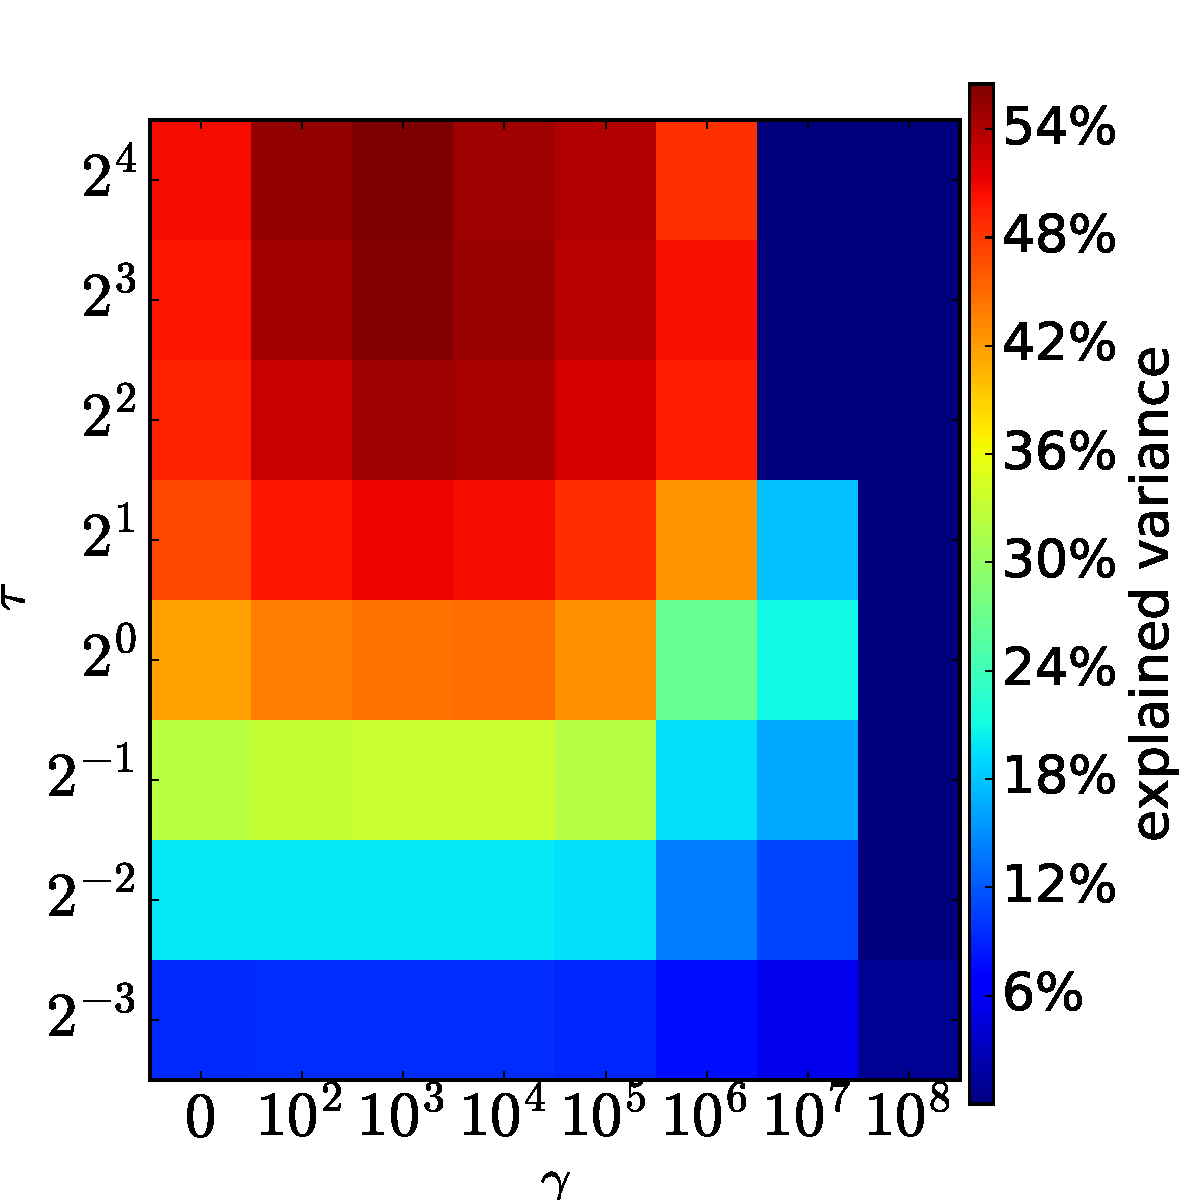
\includegraphics[width=.45\linewidth]{figures/heat_LANGUAGE_1.pdf}
%   \hspace{-.25cm}
  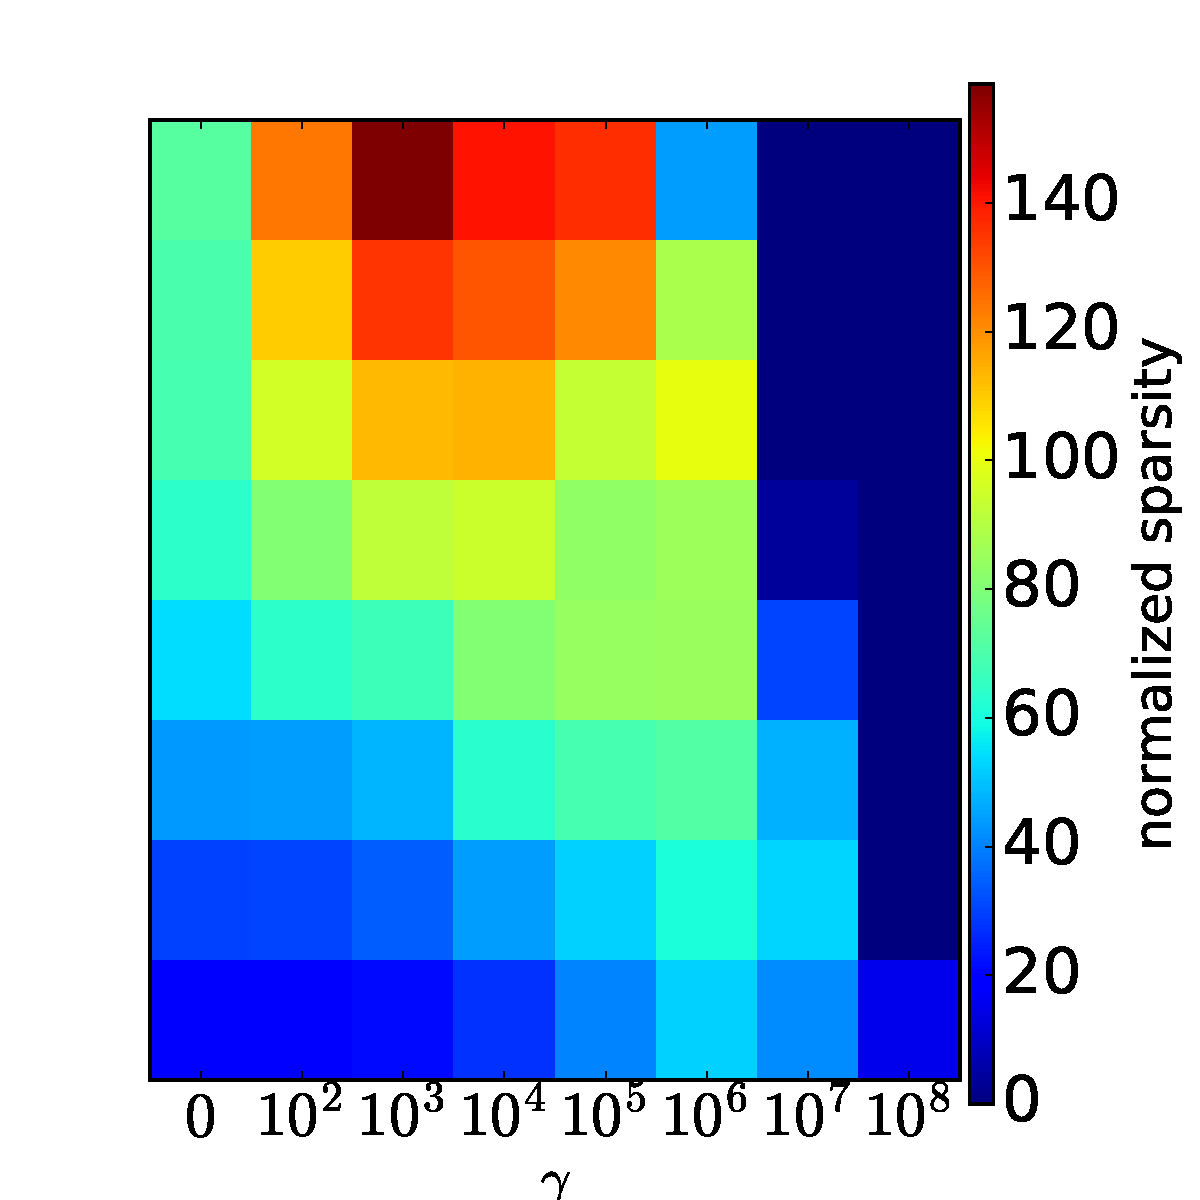
\includegraphics[width=.45\linewidth]{figures/sparsity.pdf}
  \caption{\textbf{Influence of model parameters.} %% We study the quality of the estimated dictionaries as a function of the SODL parameters $\gamma$ and $\tau$.
In the experiments, $\alpha$ was chosen according to \eqref{eq:varyingalpha}. \textbf{Left:} Percentage explained variance of the decomposition, measured on left-out data split.
    \textbf{Right: }%%  Reproducibility of the estimated across different splits of the data. %% We see that more spatial regularization (i.e larger values of $\gamma$) lead to more stable / reproducible dictionaries.
    %% \textbf{\textit{(c)}:} The average number of connected components (aka blobs) in an atom of the dictionary.
    Average normalized sparsity of the dictionary atoms. % as a function of model parameters.
  }
  % \B{d}space{-10pt}
  \label{fig:param}
\end{figure}

\paragraph*{Fidelity-stability tradeoffs.}
\textbf{Please make readbale statements. I can't help.}
Very faithful decompositions won't be stable across different splits. Also,
they will overfit on training data... There is an inherent fidelity-stability tradeoff to be made by the field practitional   \citep{abraham2013}
... See Fig. \ref{fig:param}.

Concerning the $\alpha$ parameter, inspired by   \citep{ying2006online}, we have found the following time-varying data-adaptive choice for the $\alpha$ parameter to work very well in practice:
\begin{equation}
  \alpha = \alpha_t \sim t^{-1/2}.
  \label{eq:varyingalpha}
\end{equation}
%% In the case of sparse-coding   \citep{mairal2010}, one can easily derive (see Appendix \ref{sec:alphamax}) a loose upper-bound on $\alpha$ beyond which the codes are always zero, viz:
%% \begin{equation}
%%   \alpha_{\text{max}} = \|\X\|_{\infty,\infty} := \max_{t}\|\B{x}_t\|_{\infty}.
%% \end{equation}
%% This can be useful in cross-validation.
%% In particular notice that $\alpha(t) \rightarrow 0$ as $t \rightarrow +\infty$ (i.e we can turn off regularization once ``sufficient'' data has been pooled) .
Likewise, care must be taken in selecting the Laplacian regularization parameter $\gamma$. Indeed taking it too small amounts to doing vanilla dictionary-learning model   \citep{mairal2010}. Taking it too large can lead to degenerate maps, as the spatial regularization then dominates the reconstruction error (data fidelity) term.
We find that there is a safe range of the parameter pair $(\gamma, \tau)$ in which a good compromise between the sparsity of the dictionary (thus its intepretability) and its explanation power of the data can be reached. See Fig. \ref{fig:param}.
%% This region can be found via cross-validation.
$K$-fold cross-validation with explained variance metric
%, on log-scaled grid of values verifying the upper bound \eqref{eq:blowup},
was retained as a good strategy for setting the Laplacian regularization $\gamma$ parameter and the sparsity parameter $\tau$.

% \textbf{XXX: Pending clarifications ...}

%% As a side note, if we impose and $\ell_1$ penalty on the codes instead of a Ridge, then it turns out that one can obtain a reasonable analytic upper bound for the regularization parameter $\alpha$. In did, in this case it turns out that

%% \begin{equation}
%% \text{if }  \alpha \ge \alpha_{\text{max}} := \|\X\|_{\infty,\infty} := \sup_{t \ge 0}\|\B{x}_t\|_\infty := \sup_{t \ge 0}\max_{1 \le j \le p}|\X^j_t|, \text{ then } \B{c}_t = 0,\; \forall t \ge 0.
%% \end{equation}
%% The derivation of this bound is provided in the Appendix \ref{sec:alphamax}.
%% Thus, we may only consider values of the regularization parameter in the range $0 \le \alpha \le \alpha_{\text{max}}$.

%% In 1975, Hoerl and Kennard (the original inventors of the Ridge estimator)
%% proposed to use
%% \begin{equation}
%%   \alpha_{\text{HK}} = \hat{\sigma}^2 / \max_{i}\hat{\B{c}}_i^2,
%% \end{equation}
%% where $\hat{\sigma}^2 = \|\B{x}_i - \B{D}\hat{u}_i\|_2^2 / (p - k - 1)$ is an unbiased estimate for the variance of the Ridge residuals $\r_i = \B{x}_i - \B{D}\hat{u}_i$. A simple computation shows that
%% \begin{equation}
%%   \alpha_{\text{HK}} = \mathcal O(1/p).
%% \end{equation}

%% \paragraph{Effect of the radius of the constraint set $\mathcal C$.}
%% ...

\paragraph{Initialization of the dictionary.}
Problem \eqref{eq:ss} is non-convex jointly in  $(\B{C}, \B{D})$, and so initialization might be a might be a crucial issue. However, in our experiments, we have observed that even randomly initialized dictionaries eventually produce sensible results that do not jitter much across different runs of the same experiment. %%  In our experiments on activation $Z$-maps from task fMRI contrasts (see section \ref{sec:exp}), we found that extracting blobs from the thresholded across-subject mean activation map (a relatively easy segmentation problem) and keeping the connected components which a reasonably big --say $1500\text{mm}^3$--, and then using the so-obtained regions-of-interest (ROIs) maps as initialization for the dictionary in Alg. 1 also works well in practice.
%% However we recommend the former approach, as it is more robust and needs less intervention.
%% Moreover, counting the number of these connected components yields a heuristic way to set the number of atoms $k$ in the dictionary.


\subsection{Interlude: Working in the Fourier domain (when possible)}
To close this section, let us point out a few special instances cases of problem (7), for peculiar choices of the constraint set $Q$. First note that the objective in problem (7) can be conveniently rewritten
as
\begin{equation}
  \begin{split}
    F_{\gamma\B{A}_t[j,j]^{-1}}(\B{v}, \B{V}^j + \B{A}_t[j,j]^{-1}(\B{V}\B{A}^j - \B{B}_t^j)) &=\frac{1}{2}(\B{v}-\tilde{\B{V}}^j)^T(\Id - \gamma\B{A}_t[j,j]^{-1}\Delta)(\B{v}-\tilde{\B{V}}^j)\\
    &=\frac{1}{2}(\hat{\B{v}}-\hat{\tilde{\B{V}}}^j)^T(\Id - \gamma\B{A}_t[j,j]^{-1}\Delta)(\hat{\B{v}}-\hat{\tilde{\B{V}}}^j),
  \end{split}
\end{equation}
with
  \begin{equation}
  \tilde{\B{V}}^j := (\B{A}_t[j,j]\Id -
  \gamma\Delta)^{-1}\left(\B{V}^j + \B{A}_t[j,j]^{-1}(\B{V}\B{A}^j - \B{B}_t^j)\right).
  \end{equation}

We note that the matrix-inversion $(\Id - \tilde{\gamma}\Delta)^{-1}$ that appears in the formula above is a Laplacian filter, and can
be efficiently applied in closed-form (i.e non-iteratively) in the Fourier / frequency domain. Indeed, under periodic
boundary conditions, the discrete Laplacian $\Delta$ is
Block-Circulant with Circulant Blocks (BCCB) and so is diagonalizable
in the Fourier domain. Precisely,
\begin{equation}
  \Delta = \mathcal F^*\Lambda \mathcal F
\end{equation}
where the complex orthonormal operator $\mathcal F$ represents the fast Discrete Fourier Transform (DFT), and $\Lambda$ is diagonal matrix made $p$ eigenvalues (including multiplicities) of the Laplace operator $\Delta$, given by
\begin{eqnarray*}
\begin{split}
\Lambda(\omega) &:=
-\sum_{d=1}^3\left(2\sin\left(\frac{\omega_d\pi}{2n_d}\right)\right)^2
= -2\sum_{d=1}^3\left(1-\cos\left(\frac{\omega_d\pi}{n_d}\right)
\right) \le 0,
\\
&\text{ for }\omega = (\omega_1, \omega_2, \omega_3) \in \mathbb
[\![0,n_1-1]\!] \times \mathbb [\![0,n_2-1]\!] \times [\![0,n_3-1]\!].
\end{split}
\label{eq:eigf}
\end{eqnarray*}
We note that the spectral norm of Laplace
operator in $D$ dimensions (here $D=3$) is
$\|\Delta\|_2 = \tilde{\gamma}_{\max}(-\Delta) = 2 \times D \times (1 + 1) = 4D$.

Now, one can then harvest the closed-form solution
\begin{equation}
(\Id - \tilde{\gamma}\Delta)^{-1}\a = (\mathcal F^{-1}(\Id - \tilde{\gamma} \Lambda)^{-1}\mathcal F)(\a) = \mathcal F^{-1}\left(\s\right),
\label{eq:fft}
\end{equation}
where $\s \in \mathbb R^p$ is defined by
$\s(\omega) := \dfrac{\hat{\a}(\omega)}{1-\tilde{\gamma}\hat{\Delta}(\omega)}$,
with $\hat{\a} := \mathcal F(\a)$.
These DFT computations have complexity $\mathcal O(p\log p)$.

For applying the DFTs above, one can use the FFTW\footnote{FFTW is generally taught to be one of
  the fastest implementations of the FFT, yielding up to $3 \times$ speedup against
  competing libraries like LAPACK.} --or \textit{Fastest Fourier Transform in the West}--
  library for computing the forward and inverse Fourier
  transforms needed to apply the Laplacian filter.

\paragraph{Pure $\ell_2$ constraint.}
Here, the constraint set $\mathcal C$ is an L2 ball (with radius $=1$, w.l.o.g) in $\mathbb R^2$. By the Rayleigh energy theorem (aka Parseval's identity for the DFT), one has
$$\|\hat{\B{v}}\|^2 = p\|\B{v}\|_2^2,\;\forall \B{v} \in \mathbb R^p$$ and so problem (7) can be written as
\begin{equation}
  \begin{split}
    \B{V}^j &\leftarrow \argmin_{\B{v} \in \mathbb R^p,\;\|\B{v}\|_2^2 \le 1}\frac{1}{2}(\hat{\B{v}} - \hat{\tilde{\B{V}}}^j)^*(\Id - \gamma\B{A}_t[j,j]^{-1}\Lambda)(\hat{\B{v}} - \hat{\tilde{\B{V}}}^j)\\
    &= \mathcal F^*\left(\argmin_{\hat{\B{v}} \in \mathbb C^p,\;\|\hat{\B{v}}\|_2^2 \le p}\frac{1}{2}(\hat{\B{v}} - \hat{\tilde{\B{V}}}^j)^*(\Id - \gamma\B{A}_t[j,j]^{-1}\Lambda)(\hat{\B{v}} - \hat{\tilde{\B{V}}}^j)\right)\\
    &= \mathcal F^*\left(P_{\mathcal E}(\hat{\tilde{\B{V}}}^j)\right)
  \end{split}
\end{equation}
where
\begin{equation}\mathcal E := \left\{(\Id-\gamma\B{A}_t[j,j]^{-1}\Lambda)^{\frac{1}{2}}\hat{\B{v}}\text{ s.t }\hat{\B{v}} \in \mathbb C^p,\;\|\hat{\B{v}}\|_2^2 \le p\right\},
\end{equation}
a hyper-ellipsoid in standard position (i.e $\mathbf{0}$-centered and axes-aligned). Using elementary geometric arguments, one can show that the projection $P_{\mathcal E}(\hat{\tilde{\B{V}}}^j)$ can be computed efficiently using a kind of root-finding algorithm \cite{Dai06}, and converges exponentially fast.

\paragraph{Non-negative Lasso.}
In case the constraint set $\mathcal C$ for the dictionary atoms is a
simplex $\mathcal S_p(\tau)$, the simplex (see section \ref{sec:contrib}), then the BCD update for the $j$th atom becomes
\begin{equation}
  \begin{split}
    \B{V}^j &\leftarrow \argmin_{\B{v} \in \mathbb R^p,\;\B{v} \ge 0,\;\1^T\B{v} \le 1}\frac{1}{2}(\hat{\B{v}} - \hat{\tilde{\B{V}}}^j)^*(\Id - \gamma\B{A}_t[j,j]^{-1}\Lambda)(\hat{\B{v}} - \hat{\tilde{\B{V}}}^j)\\
    &= \mathcal F^*\left(\argmin_{\hat{\B{v}} \in \mathbb C^p,\;-\mathcal F^*\hat{\B{v}} \le 0,\; \hat{\1}^T\hat{\B{v}} \le 1}\frac{1}{2}(\hat{\B{v}} - \hat{\tilde{\B{V}}}^j)^*(\Id - \gamma\B{A}_t[j,j]^{-1}\Lambda)(\hat{\B{v}y} - \hat{\tilde{\B{V}}}^j)\right),
  \end{split}
\end{equation}
which is a diagonal quadratic program with linear constraints, and can be effectively solved via the well-known simplex method, for example.


\section{Related works}
%% To the best of our knowledge, dictionary-learning techniques for fMRI
%% space-time decompositions were historically introduced by
%%   \citep{varoquaux2011}.
While there exist algorithms for online sparse dictionary-learning
that are very efficient in large-scale settings (for example
  \citep{mairal2010}, or more recently   \citep{mensch2016dictionary})
imposing spatial structure introduces
couplings in the corresponding optimization problem   \citep{dohmatob2014benchmarking}. So far,
spatially-structured decompositions have been solved by very slow
alternated optimization   \citep{varoquaux2011,abraham2013}. Notably,
structured priors such as TV-$\ell_1$   \citep{baldassarre2012} minimization,
were used by   \citep{abraham2013} to extract data-driven
state-of-the-art atlases of brain function.
However, alternated minimization is very slow, and large-scale medical
imaging has shifted to online solvers for
dictionary-learning like   \citep{mairal2010} and   \citep{mensch2016dictionary}.
%
These do not readily
integrate structured penalties. As a result, the use of structured
decompositions has been limited so far, mostly due to the computational
cost of the ensuing algorithms. 
%
Our approach instead uses a Laplacian penalty to impose spatial
structure at a very minor cost and adapts the online-learning
dictionary-learning framework   \citep{mairal2010}, resulting in a fast
and scalable structured decomposition.
%
Second, the approach in   \citep{abraham2013} though very novel, is
heuristic, as it does not come with theoretical guarantees. In contrast, our
method enjoys the same convergence guarantees and comparable numerical
complexity as the basic unstructured online dictionary-learning
  \citep{mairal2010}.

Finally, one should also mention   \citep{varoquaux2013cohort} that introduced an online group-level functional brain mapping strategy for differentiating regions reflecting the variety of brain network configurations observed a
the population, by learning a sparse-representation of these in the spirit of   \citep{mairal2010}.
%% Finally, it is worth mentioning an optimized version   \citep{mensch2016dictionary} of   \citep{mairal2010} which has recently appeared, wherein the authors combine \textit{sketching} techniques (precisely, they randomly sub-sample the brain images over both space and time) with online dictionary-learning to obtain an algorithm which can scale to tera-bytes of data, without degrading the quality of the estimated dictionary.

%% The Laplacian penalty penalty  can imposes smoothnes on the dictionary atoms at a very minor cost.
%% To the best of our knowledge, dictionary-learning techniques for fMRI
%% space-time decompositions were historically introduced by
%%   \citep{varoquaux2011},
%% using alternated minimization and a smoothness penalty.
%% Indeed, in such an alternate optimization --a block coordinate descent
%% optimizing separately for both matrices in the factorization-- proximal
%% operator can be used to impose structured penalties
%%   \citep{jenatton2010structured}.

%% One should also mention   \citep{abraham2013}, wherein the TV prior, which is very different from Laplacian prior, was  used to impose spatial structure. The TV prior, though it is known to have some qualitative advantages over Laplacian regularization (e.g the former enforces boundaries in the maps), is neither differentiable nor proximable analytically. Laplacian prior leads to much easier problems. Second, the approach in   \citep{abraham2013} though very novel, is grossly heuristic: it lacks theoretical justification and tight links to technical literature. In contrast, our method enjoys the same convergence guarantees and comparable numerical complexity as the basic unstructured online dictionary-learning   \citep{mairal2010}.
%% The Laplacian penalty penalty 
%% can imposes smoothness on the dictionary atoms at a very minor cost.
%

\section{Experiments}
\label{sec:exp}
\paragraph*{Setup.} Our experiments were done on task fMRI data from $500$ subjects
from the HCP --Human Connectome Project-- dataset
  \citep{VanEssen20122222}. These task fMRI data were acquired in an
attempt to assess major domains that are thought to sample the
diversity of neural systems of interest in functional connectomics.
%  including: 1) visual, motion,
% somatosensory, and motor systems; 2) language processing (semantic and
% phonological processing); 3) social cognition (Theory of Mind); and 4)
% emotion processing...
We studied the activation maps related to a task that involves
language (story understanding) and mathematics (mental
computation). This particular task is expected to outline number, attentional and
language networks, but the variability modes observed in the
population cover even wider systems. For the experiments,
mass-univariate  General Linear Models (GLMs)   \citep{friston1995} for
$n=500$ subjects
were estimated for the \emph{Math vs Story} contrast (language
protocol), and the corresponding full-brain $Z$-score maps each
containing $p=2.6 \times 10^5$ voxels, were used as the input data $\X \in
\mathbb R^{n \times p}$,  and we
sought a decomposition into a dictionary of $k = 40$ atoms (components).
The input data $\X$ were shuffled and then split into two groups of the same
size.

\paragraph*{Models compared and metrics.} We compared our proposed Smooth-SODL model \eqref{eq:ss} against both the Canonical ICA --CanICA   \citep{varoquaux2010group}, a single-batch multi-subject PCA/ICA-based method, and the standard SODL (sparse online dictionary-learning)   \citep{mairal2010}. While the CanICA model accounts for subject-to-subject differences, one of
its major limitations is that it does not model spatial variability across
 subjects. Thus we estimated the CanICA components on smoothed data: isotropic FWHM of 6mm, a necessary preprocessing step for such methods. In contrast, we did no pre-smoothing for the SODL of Smooth-SODL models.
The different models were compared across a variety of qualitative and quantitative metrics: visual quality of the dictionaries obtained, explained variance, stability of the dictionary atoms, their reproducibility, performance of the dictionaries in predicting behavioral scores (IQ, picture vocabulary, reading proficiency, etc.) shipped with the HCP data   \citep{VanEssen20122222}. For both SODL  \citep{mairal2010} and our proposed Smooth-SODL model, the constraint set for the dictionary atoms was taken to be a simplex $\mathcal C := \mathcal S_p(\tau)$ (see section \ref{sec:contrib} for definition). The results of these experiments are presented in Fig. \ref{fig:maps}
and \ref{fig:ev}.

\section{Results}
\label{sec:results}
\paragraph{Qualitative assessment of dictionaries.}
As can be seen in Fig. \ref{fig:maps}\textit{(a)}, all methods recover
dictionary atoms that represent known functional brain organization;
notably the dictionaries all
contain the well-known executive control and attention networks, at least
in part. Vanilla dictionary-learning leverages the denoising properties
of the $\ell_1$ sparsity constraint, but the voxel clusters are not very structured. For, example most blobs are surrounded with a thick ring of very small nonzero values.  In contrast, our proposed regularization model leverages both sparse and structured dictionary atoms, that are more spatially structured and less noisy.

In contrast to both SODL and Smooth-SODL, CanICA   \citep{varoquaux2010group} is an ICA-based method which enforces no notion of sparsity whatsoever. The result are therefore dense and noisy dictionary atoms that explain the data very well (Fig. \ref{fig:maps}\textit{(b)} but which are completely unintepretable. In a futile attempt to remedy the situation, in practice such PCA/ICA-based methods (including FSL's MELODIC tool   \citep{smith2004advances}) are hard-thresholded in order to see information. For CanICA, the hard-thresholded version has been named tCanICA in Fig. \ref{fig:maps}.
That notwithstanding, notice how the major structures (parietal lobes, sulci, etc.) in each atom are reproducible across the different models.

  
\begin{figure}[!htb]
%%   \includegraphics[width=.24\linewidth]{{rpca_nc=20_0}.png}
%%   \hspace{-.5em}
%%   \includegraphics[width=.24\linewidth]{{rpca_nc=20_1}.png}
%%     \hspace{-.5em}
%%     \includegraphics[width=.24\linewidth]{{rpca_nc=20_2}.png}
%%       \hspace{-.5em}
%%       \includegraphics[width=.24\linewidth]{{rpca_nc=20_3}.png}
%% \subfigure [PCA components, thresholded to keep only top 90\% voxels] {
%%   \includegraphics[width=.24\linewidth]{{rpca_nc=20_12}.png}
%%     \hspace{-.5em}
%%     \includegraphics[width=.24\linewidth]{{rpca_nc=20_13}.png}
%%       \hspace{-.5em}
%%       \includegraphics[width=.24\linewidth]{{rpca_nc=20_14}.png}
%%         \hspace{-.5em}
%% \includegraphics[width=.24\linewidth]{{rpca_nc=20_15}.png}
  %% }

  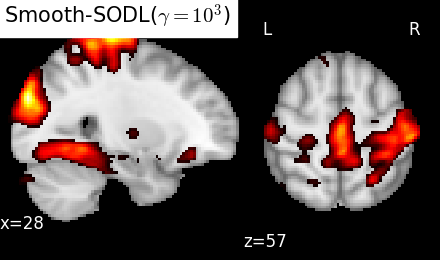
\includegraphics[width=0.244\linewidth]{{figures/components_LANGUAGE_nc=40_alpha=auto_gamma=1000_radius=4_split=0_time=12_3}.png}
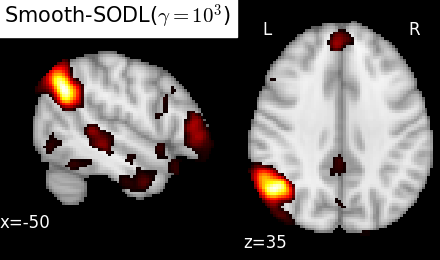
\includegraphics[width=0.244\linewidth]{{figures/components_LANGUAGE_nc=40_alpha=auto_gamma=1000_radius=4_split=0_time=12_29}.png}
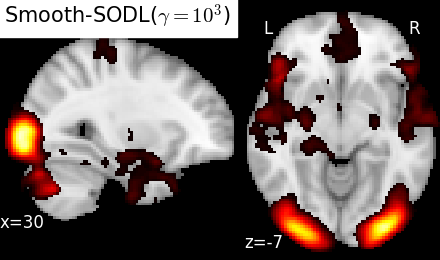
\includegraphics[width=0.244\linewidth]{{figures/components_LANGUAGE_nc=40_alpha=auto_gamma=1000_radius=4_split=0_time=12_36}.png}
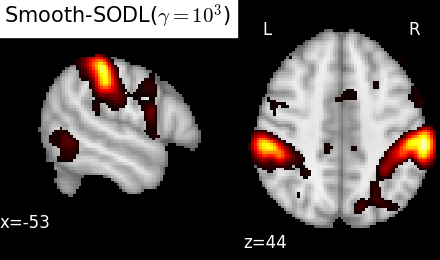
\includegraphics[width=0.244\linewidth]{{figures/components_LANGUAGE_nc=40_alpha=auto_gamma=1000_radius=4_split=0_time=12_39}.png}

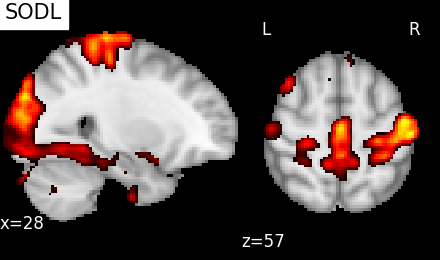
\includegraphics[width=0.244\linewidth]{{figures/components_LANGUAGE_nc=40_alpha=auto_gamma=0_radius=4_split=0_time=12_34}.png}
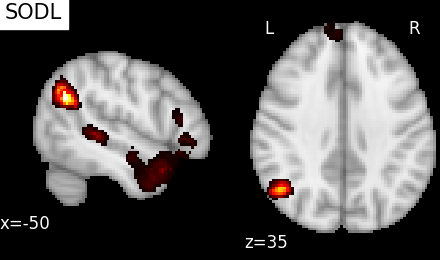
\includegraphics[width=0.244\linewidth]{{figures/components_LANGUAGE_nc=40_alpha=auto_gamma=0_radius=4_split=0_time=12_29}.png}
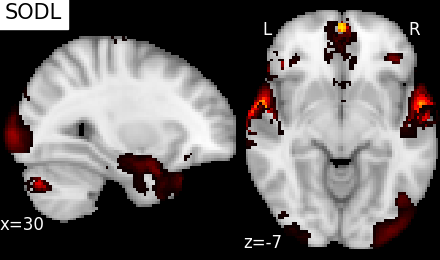
\includegraphics[width=0.244\linewidth]{{figures/components_LANGUAGE_nc=40_alpha=auto_gamma=0_radius=4_split=0_time=12_37}.png}
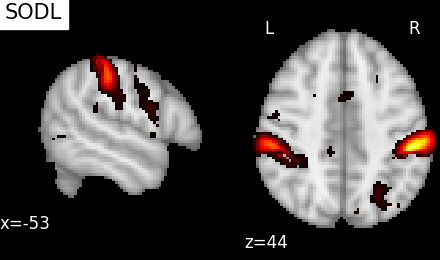
\includegraphics[width=0.244\linewidth]{{figures/components_LANGUAGE_nc=40_alpha=auto_gamma=0_radius=4_split=0_time=12_3}.png}

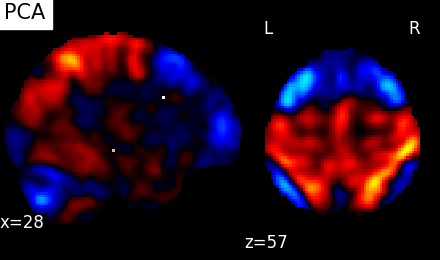
\includegraphics[width=0.244\linewidth]{{figures/components_LANGUAGE_nc=40_PCA_2}.png}
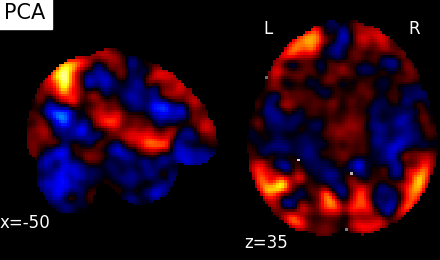
\includegraphics[width=0.244\linewidth]{{figures/components_LANGUAGE_nc=40_PCA_7}.png}
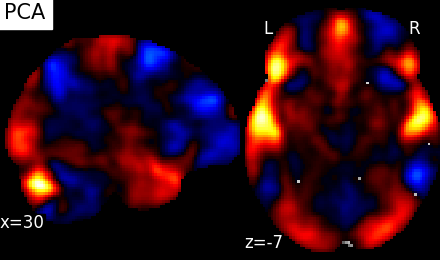
\includegraphics[width=0.244\linewidth]{{figures/components_LANGUAGE_nc=40_PCA_1}.png}
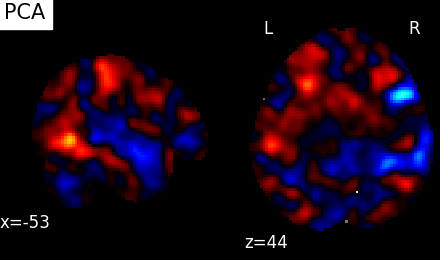
\includegraphics[width=0.244\linewidth]{{figures/components_LANGUAGE_nc=40_PCA_26}.png}

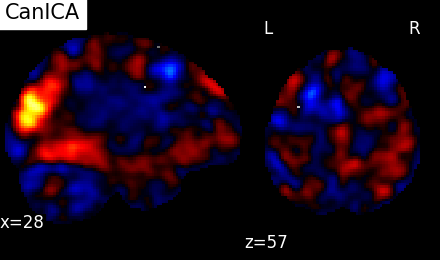
\includegraphics[width=0.244\linewidth]{{figures/components_LANGUAGE_nc=40_CanICA_26}.png}
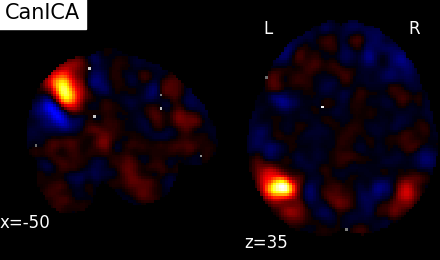
\includegraphics[width=0.244\linewidth]{{figures/components_LANGUAGE_nc=40_CanICA_28}.png}
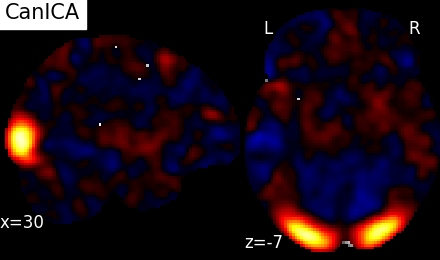
\includegraphics[width=0.244\linewidth]{{figures/components_LANGUAGE_nc=40_CanICA_23}.png}
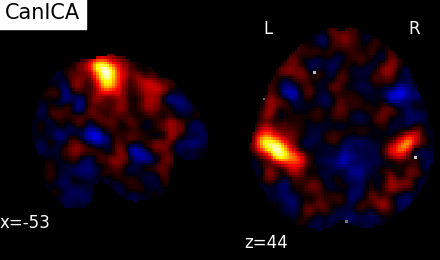
\includegraphics[width=0.244\linewidth]{{figures/components_LANGUAGE_nc=40_CanICA_24}.png}
% \begin{subfigure}[t]{1\linewidth}
%   \centering
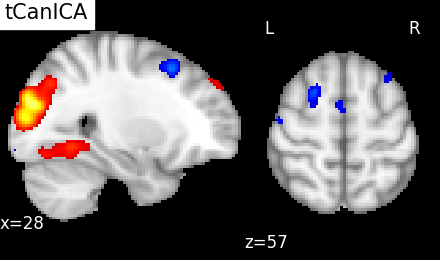
\includegraphics[width=0.244\linewidth]{{figures/components_LANGUAGE_nc=40_tCanICA_26}.png}
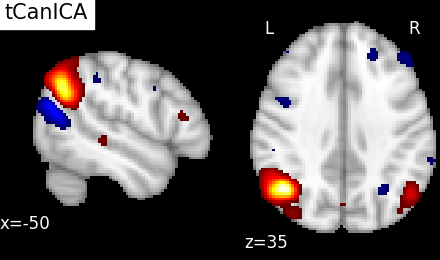
\includegraphics[width=0.244\linewidth]{{figures/components_LANGUAGE_nc=40_tCanICA_28}.png}
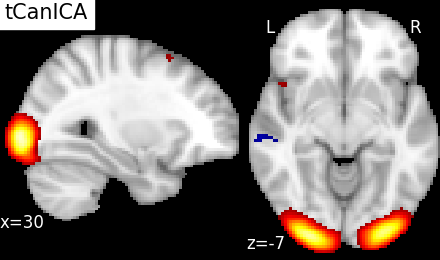
\includegraphics[width=0.244\linewidth]{{figures/components_LANGUAGE_nc=40_tCanICA_23}.png}
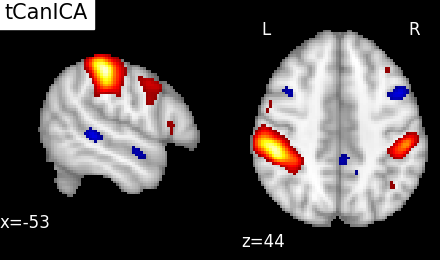
\includegraphics[width=0.244\linewidth]{{figures/components_LANGUAGE_nc=40_tCanICA_24}.png}
\caption{\textbf{Qualitative comparison of the estimated dictionaries.} Each column represents an atom of the estimated dictionary, where atoms from
  the different models (the rows of the plots) have been matched via a Hungarian algorithm. Here, we only show a limited number of the most ``intepretable'' atoms. Notice how the major structures in each atom are reproducible across the different models. %% We see that our proposed approach produces more structured dictionaries: the atoms are well-segmented piece-wise smooth and compact, making up blobs, as opposed to scattered patterns of activation.
  Maps corresponding to hard-thresholded CanICA
    \citep{varoquaux2010group} components have also been included, and have been called tCanICA. In contrast, the maps from the SODL   \citep{mairal2010} and our proposed Smooth-SODL \eqref{eq:ss} were not been thresholded.
 }
   
% \end{subfigure}
% ~
% \begin{subfigure}[c]{.66\linewidth}
%   \centering

  ~~~~
%  \begin{minipage}{.9\linewidth}
%   \end{minipage}
% \end{subfigure}

% \caption{\textbf{Main results.} Benchmarking our proposed Smooth-SODL \eqref{eq:ss} model against competing state-of-the-art methods like SODL (sparse online dictionary-learning)   \citep{mairal2010} and CanICA   \citep{varoquaux2010group}.}
\label{fig:maps}
\end{figure}


\paragraph{Stability-fidelity trade-offs.}
PCA/ICA-based methods like CanICA   \citep{varoquaux2010group} and MELODIC   \citep{smith2004advances} are the optimal linear decomposition method to maximize
explained variance on a dataset. On the training set,  CanICA   \citep{varoquaux2010group} out-performs all
others algorithms with about 66\% (resp. 50\% for SODL  \citep{mairal2010} and 58\% for Smooth-SODL) of explained variance on the training set, and 60\% (resp. 49\% for SODL and \textbf{55\%} for Smooth-SODL) on left-out (test) data. See Fig. \ref{fig:maps}\textit{(b)}. However, as noted in the above paragraph, such methods lead to dictionaries that are hardly intepretable and thus the user must
% invariably
recourse to some kind of post-processing hard-thresholding step, which destroys the estimated model. More so,
assessing the stability of the dictionaries, measured by mean correlation between corresponding atoms, across different splits of the data, CanICA   \citep{varoquaux2010group} scores a meager 0.1, whilst the hard-thresholded version tCanICA obtains 0.2, compared to \textbf{0.4} for Smooth-SODL and 0.1 for SODL.   As is to be expected, notice how the RAW model over-fits.
The voxel space of worth $p=261596$ voxels is reduced to $k=40$ components, and then each subject $Z$-map $\B{x}_t$ of worth $p=261596$ voxels is reduced to $k=40$ coefficients via a simple ridge regression \eqref{eq:coding}.

 \begin{figure}[!htpb]
   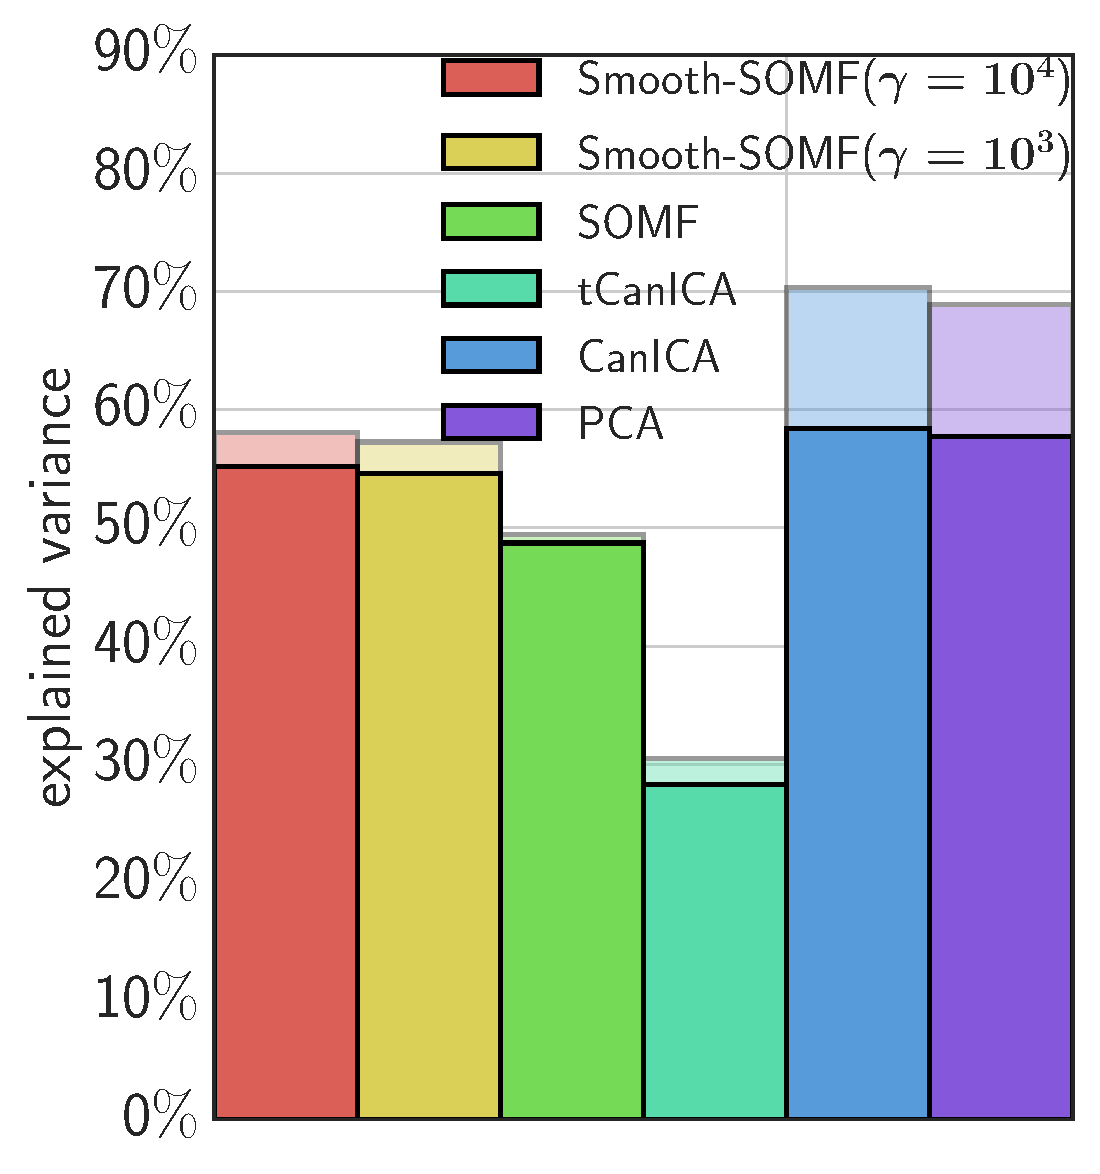
\includegraphics[width=.35\linewidth]{ev_scores_LANGUAGE.pdf}
   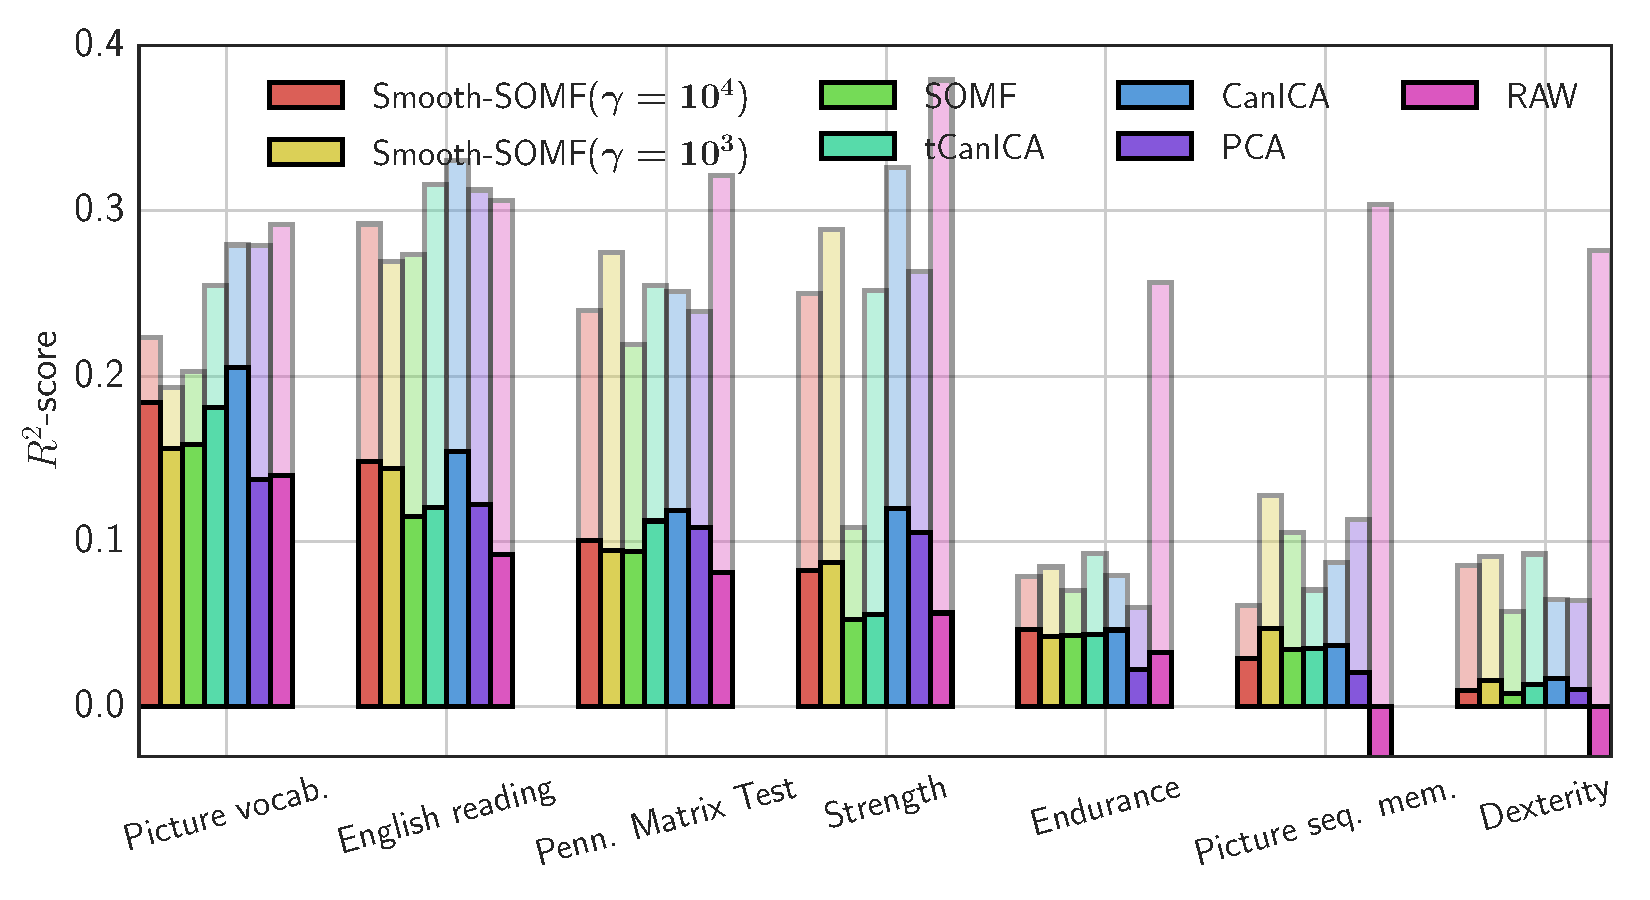
\includegraphics[width=.65\linewidth]{behavioral_scores_LANGUAGE.pdf}  

   \caption{\textbf{Left:} Mean explained variance of the different models on both training data and test (left-out) data. \textbf{N.B.:} Bold bars represent performance on \textbf{test} set while faint bars in the 
  background represent performance on \textbf{train} set. 
  \textbf{Right:} Predicting  behavioral  variables of the HCP  \citep{VanEssen20122222} dataset using subject-level $Z$-maps.
  }
  \end{figure}


\paragraph{Prediction of behavioral variables.}
If Smooth-SODL captures the patterns of inter-subject variability, then it should be possible to predict cognitive scores $\y$ like picture vocabulary, reading proficiency, math aptitude, etc. (the behavioral variables are explained in the HCP wiki   \citep{hcpwiki}) by projecting new subjects' data into this learned low-dimensional space (via solving the ridge problem \eqref{eq:coding} for each sample $\B{x}_t$), without loss of performance compared with using the raw $Z$-values values $\X$. Let RAW refer to the direct prediction of targets $\y$ from $\X$, using the top 2000 most voxels most correlated with the target variable. Results of for the comparison are shown in Fig. \ref{fig:maps}\textit{(c)}.  Only variables predicted with a a positive mean (across the different methods and across subjects) $R$-score are reported.
%% Indeed, prediction results (Fig. \ref{fig:results}) show that the enhanced dictionaries obtained by our proposed method ($\gamma > 0$) is not at the expense of a decreased predictive power.
We see that the RAW model, as expected over-fits drastically, scoring an $R^2$ of 0.3 on training data and only 0.14 on test data. Overall, for this metric CanICA performs best than all the other models in predicting the different behavioral variables on test data. However, our proposed Smooth-SODL model outperforms both SODL   \citep{mairal2010} and tCanICA, the thresholded version of CanICA.

  
\paragraph{Running time.} On the computational
side, the vanilla dictionary-learning
SODL algorithm   \citep{mairal2010} with a batch size of
$\eta = 20$ took about $110$s ($\approx 1.7$ minutes) to
run, whilst with the same batch size, our proposed
Smooth-SODL model \eqref{eq:ss} implemented in Alg. \ref{Tab:algo} took
$340$s ($\approx 5.6$ minutes), which is slightly less than \textbf{3 times}
slower than SODL.  Finally, CanICA   \citep{varoquaux2010group} for this experiment
took $530$s ($\approx 8.8$ minutes) to run, which is about \textbf{5 times} slower
than the SODL model and \textbf{1.6 times} slower than our proposed Smooth-SODL
\eqref{eq:ss} model.
All experiments were run on a single CPU of a modern laptop.

        
\paragraph{Is spatial regularization really needed ?}
Ideally, one does not need spatial regularization if data are abundant (like in the HCP). So we computed learning curves of mean explained variance (EV) on test data, as a function of the amount training data seen by both Smooth-SODL and SODL   \citep{mairal2010} (Fig. \ref{fig:ev}).
In the beginning of the curve, our proposed spatially regularized Smooth-SODL model starts off with more than 31\% explained variance (computed on 241 subjects), after having pooled only 17 subjects. In contrast, the vanilla SODL model   \citep{mairal2010} scores a meager 2\% explained variance; this corresponds  to a 14-fold gain of Smooth-SODL over SODL. As more and more that are pooled, both models explain more variance, and the gap between Smooth-SODL and SODL reduces, and both models perform comparably asymptotically. % (i.e the gain factor tends to $1$).

\begin{figure}[!htp]
 \begin{tabular}{|c|c|c|c|c}\hline%\hline
    {Nb. subjects pooled} & {vanilla SODL} & {proposed model} & {gain factor} \\ \hline
17 & {2\%} & \bf{31\%} & {x13.8}\\\hline
92 & 37\% & \bf{50\%} & x1.35\\\hline
167 & 47\% & \bf{54\%} & x1.15\\\hline
241 & 49\% & \bf{55\%} & x1.11\\
  \end{tabular}
 \caption{\textbf{Learning-curve} for boost in explained variance of our proposed Smooth-SODL model over the reference SODL model.
   Note the reduction in the gain in EV as more data are pooled.}
 \label{fig:ev}
\end{figure}


% %% \begin{itemize}
% %%   \item With 19 subjects: mean explained variance for SODL = 0.87\%; mean explained variance for Smooth-SODL = 33.57\%; gain factor = \textbf{38x} (significance: $p < 10^{-6}$)
% %% \item With 112 subjects: mean explained variance for SODL = 33.98\%; mean explained variance for Smooth-SODL = 41.88\%; gain factor = \textbf{1.23x} (significance: $p < 10^{-6}$)
% %% \item With 241 subjects: mean explained variance for SODL = 41.85\%; mean explained variance for Smooth-SODL = 44.83\%; gain factor = \textbf{1.07x} (significance: $p < 2\times 10^{-5}$).
% %% \end{itemize}
% Thus our proposed Smooth-SODL method extracts structured denoised dictionaries that better capture inter-subject variability in small, medium, and large-scale regimes alike.

\section{Concluding remarks}
To extract structured functionally discriminating patterns
from massive brain data (i.e data-driven atlases), we have extended
the online dictionary-learning framework first developed in
  \citep{mairal2010}, to learn structured regions
representative of brain organization. To this end, we have successfully augmented   \citep{mairal2010} with a Laplacian prior on the component maps,
while conserving the low numerical complexity of the latter.
Through experiments, we have shown that the resultant model --Smooth-SODL model \eqref{eq:ss}-- extracts structured and denoised dictionaries that are more intepretable and better capture inter-subject variability in small medium, and large-scale regimes alike, compared to state-of-the-art models.
We believe such online multivariate online methods shall become the de facto
way do dimensionality reduction and ROI extraction in future.

\paragraph{Extensions.} One can envisage to replace the Laplacian regularization with a general structure-inducing penalty for which the proximal operator is easy to compute. Such a framework is developed in chapter \ref{chap:proxdict}, and produces an entire family models, with potentially different properties.


\paragraph{Implementation.} The authors' implementation of the proposed
SS0MF \eqref{eq:ss} model will soon be made available as part of the
\textit{Nilearn} package   \citep{nilearn}.


% \newglossaryentry{MRI}{name=MRI,description={{Magnetic Resonance Imaging}}}



% The primary form of fMRI measures the oxygen change in blood flow. This is known as the Blood-oxygen-level dependent (BOLD) contrast. Other increasingly popular functional MRI method is arterial spin labeling (ASL)~ \citep{detre1994tissue, alsop1998multisection, williams1992magnetic}, which uses arterial water as tracer to measure cerebral blood flow. Compared to fMRI, ASL has a lower signal to noise ratio~ \citep{detre2002technical}. However, ASL provides reliable absolute quantification of cerebral blood flow with higher spatial and temporal resolution than other techniques~ \citep{borogovac2012arterial}. This thesis specifically considers BOLD functional MRI and through the manuscript we use the name functional MRI (fMRI) to denote functional MRI based on the BOLD signal.

% \newglossaryentry{bold}{name=BOLD,description={{fMRI contrast that measures oxygen change in blood flow}}}

% %
% The \emph{\gls{bold}} contrast can be explained by considering a protein present in
% the blood
% cells, called hemoglobin. Hemoglobin can bind with oxygen in order to bring it
% into the different cells of the organism, this link being reversible and
% unstable. Thus, it can be found in two different forms: \emph{oxyhemoglobin}
% ($Hb-O_{2}$ - giving a bright red color to the blood), its oxygenated form, and
% \emph{deoxyhemoglobin} ($Hb$ - giving a blue-purple color to the blood), its
% deoxygenated form.
% %
% %
% %
% %
% When the \emph{oxyhemoglobin} loses its oxygen atoms and
% becomes the \emph{deoxyhemoglobin}, it becomes more affected by an externally applied magnetic field (due to the iron
% oxides). The presence of
% \emph{deoxyhemoglobin} in the blood modifies the
% magnetic resonance signal of the protons of the water molecules surrounding the blood
% vessels. 

% \begin{figure}
% \centering
% \includegraphics[width=1.\linewidth]{chapter_1/chapter_1_bold.png}
% \caption[][-2.5cm]{
% Illustration of the effect of the $CO_2$ on the \emph{BOLD} contrast.
% Left - Coronal slice showing the \emph{BOLD} contrast of an anesthetized rat
% which has breathed pure $O_2$. Right - Coronal slice of the same rat, showing the \emph{BOLD} contrast after respiration of a mixture of $90\%$ of $O_2$ and $10\%$ of $CO_2$ (this mixture
% increases the oxygenation of the venous blood). The arrow shows 
% the sagittal sinus, which is one of the major veins of the brain. This picture shows a strong increase of intensity in this vein, that illustrates that the
% variation of blood oxygenation is visible in \emph{BOLD} contrast.
% Adapted from  \citep{ogawa1990b}.}\label{fig:chapter_1_ogawa}
% \end{figure}


% The difference of magnetic
% susceptibility between the
% blood vessel and the surrounding tissues creates 
% inhomogeneities in the magnetic field  \citep{thulborn1982,ogawa1990a} that are quantified by the magnetic resonance scanner. In the seminal paper  \citep{ogawa1990b} studied the variations of
% \emph{BOLD} contrast in the brain of an anesthetized rat during the inhalation of a gas
%  that increases the \emph{cerebral blood flow} (\emph{CBF}), and thus blood
% oxygenation (see Figure
% \ref{fig:chapter_1_ogawa}).

% \newglossaryentry{voxel}{name={voxel},description={unity of measure in a volumetric space}}
% \newglossaryentry{TR}{name={TR},description={repetition time, sampling time in an fMRI scanner}}

% The spatial resolution is given by the size of a \emph{\gls{voxel}}, a three-dimensional rectangular cuboid given by a single measure of the scanner. Voxel sizes range from 4mm to 1mm. Smaller voxels contain fewer neurons on average, incorporate less blood flow and hence have less signal to noise ratio than larger voxels. Smaller voxel size also makes up for longer acquisition time since this is proportional to the number of voxels per slice and the number of slices to scan. 

% The time resolution of an fMRI scanner is given by the repetition time (\gls{TR}) of successive image acquisitions. A slice of the volume acquisition has an acquisition window that is about 20-30ms in duration. For example, in the study~ \citep{borghesani:hal-00986606} we used voxel sizes of $1.5 \times 1.5 \times 1.5$mm, 82 slices and a repetition time (TR) of 2.3 seconds for a full-brain coverage. These number are for routine fMRI, however it is possible to change the tradeoff between spatial and temporal resolution. With the advent of compressed sensing techniques for faster acquisition times~ \citep{MRM:MRM21391, Zong2014312, chauffertvariable} and the deployment of scanners with fields of 7-Tesla and beyond~ \citep{hanke2014high} these numbers are likely to change in the near future.

% % The dynamics, location, and magnitude of the signal are highly influenced by the vasculature as it is sampled in each voxel. If a voxel happen to capture large vessel effects, the magnitude of the signal may be larger, the timing a bit more delayed than average (up to 4 s delayed from capillary effects)~ \citep{bandettini2009functional}

% \clearpage
\bibliographystyle{plainnat}
\bibliography{bib_all}
